یک نمونه از الگوریتم‌های جستجو محلی آن است که state بعدی را کاملا به صورت رندوم از میان state های حالت فعلی بدست آوریم \\ ( walk random ) و یا آنکه در هر مرحله یک state از مسئله را کاملا به صورت تصادفی انتخاب کنیم.( sampling random )

نکته مهم در مورد این دو روش آن است که هردو آنها در زمان بینهایت complete هستند.
به عبارتی در space محدود، هر state از مسئله visit می‌شود.

\begin{figure}[H]
    \centering
    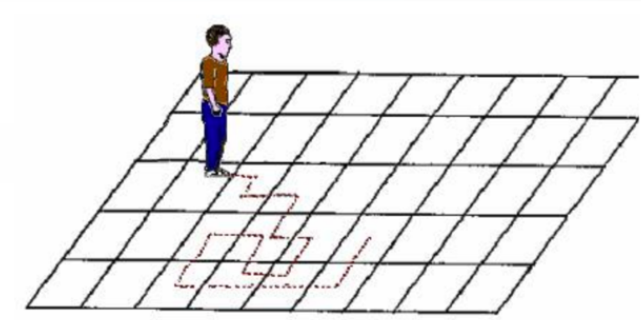
\includegraphics[width=0.8\linewidth]{source/random-walk.png}
    \label{fig:random-walk}
\end{figure}